Training of the five RGB backbones across the four main experiments is complete, with two additional probes reported below: a frequency-only ResNet-18 baseline and a no-retraining score-level temporal aggregation baseline. Unless stated, all reported values are video-level. Table~\ref{tab:main_auc} gives the primary AUC results; complete accuracy, F1, EER, confusion matrices, manipulation breakdowns, and pairwise-test tables appear in Online Resource~1.

\begin{table*}[!t]
\caption{Video-level AUC with 95\% bootstrap confidence intervals. Bold marks the highest point estimate in each experiment; it does not imply statistically significant superiority.}
\label{tab:main_auc}
\centering
\scriptsize
\setlength{\tabcolsep}{2pt}
\resizebox{\textwidth}{!}{%
\begin{tabular}{lcccc}
\toprule
Backbone & Exp1: FF++$\to$FF++ & Exp2: FF++$\to$Celeb-DF & Exp3: Celeb-DF$\to$FF++ & Exp4: Mixed$\to$DFD \\
\midrule
EfficientNet-B4 & 0.900 (0.85--0.94) & 0.713 (0.63--0.80) & 0.506 (0.47--0.54) & 0.788 (0.75--0.82) \\
Xception & 0.736 (0.65--0.81) & 0.573 (0.47--0.67) & 0.543 (0.51--0.57) & 0.735 (0.70--0.77) \\
ResNet-50 & 0.924 (0.88--0.97) & 0.799 (0.72--0.87) & \textbf{0.589 (0.56--0.62)} & 0.812 (0.78--0.84) \\
ConvNeXt-Tiny & \textbf{0.957 (0.92--0.99)} & \textbf{0.806 (0.72--0.88)} & 0.576 (0.54--0.61) & \textbf{0.915 (0.89--0.93)} \\
ViT-Base & 0.867 (0.80--0.93) & 0.668 (0.57--0.76) & 0.588 (0.56--0.62) & 0.713 (0.67--0.75) \\
\botrule
\end{tabular}%
}
\end{table*}

\subsubsection{Backbone comparison and transfer}
I read the numbers in Table~\ref{tab:main_auc} as point estimates first, then examine the reported paired comparisons, subject to the empirical bootstrap-tail limitations in Online Resource~1. ConvNeXt-Tiny and ResNet-50 have the two highest observed AUCs in Exp1, Exp2, and Exp4. Their difference is not significant after Holm adjustment in Exp1 ($q_{\mathrm{boot}}=0.147$, $q_{\mathrm{McN}}=0.688$) and is negligible in Exp2 ($\Delta\mathrm{AUC}=0.007$, $q_{\mathrm{boot}}=0.875$). I therefore report ConvNeXt-Tiny as the strongest observed point estimate, not as a uniquely superior architecture. ViT-Base does not lead under this common recipe. Because the five backbones share one baseline pipeline, the comparison should be read as a comparison under that recipe rather than as an optimization of each architecture's training strategy.

Every backbone degrades from the in-distribution setting to the cross-dataset settings, so the in-domain numbers overstate deployment performance. FF++$\to$Celeb-DF and Mixed$\to$DFD retain useful discrimination, whereas the reverse Celeb-DF$\to$FF++ transfer is weakest (AUC 0.506--0.589). ResNet-50's confidence interval in Exp3 lies above 0.5, so I describe this setting as weak or near-chance rather than uniformly at chance. Within this protocol, the asymmetry is consistent with source-domain coverage contributing to the result. However, dataset size, manipulation families, identities, and acquisition pipelines are confounded, so this interpretation should not be treated as a causal finding.

Figure~\ref{fig:generalization_summary} summarizes the cross-dataset means and the range across backbones for the four experiments.

\begin{figure*}[!t]
\centering
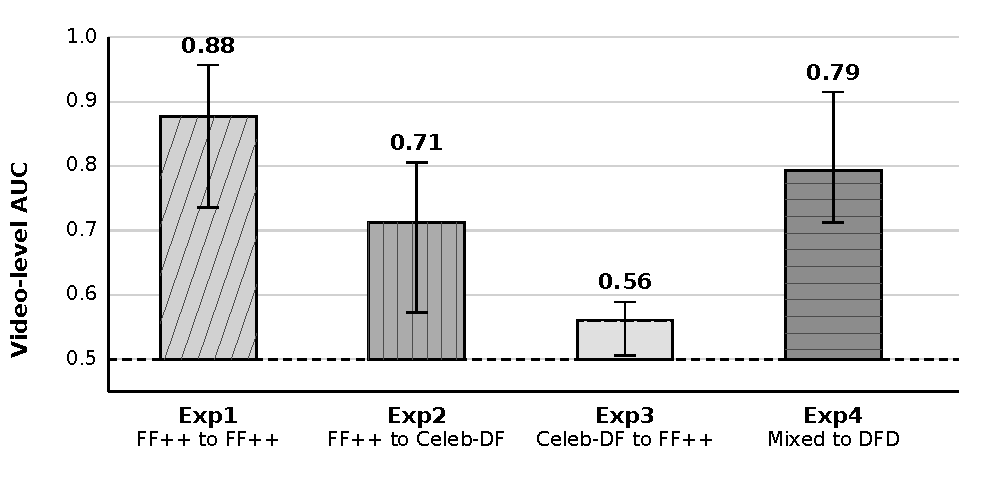
\includegraphics[width=0.92\textwidth]{Fig2.pdf}
\caption{Cross-dataset summary of Table~\ref{tab:main_auc}. Bars are means over the five backbones, whiskers show their minimum--maximum range, and the dashed line marks chance AUC}
\label{fig:generalization_summary}
\end{figure*}

\subsubsection{Diagnostic probes and robustness}
Table~\ref{tab:compact_diagnostics} keeps the diagnostic results most relevant to the central conclusion. The no-progressive-unfreezing configuration improves EfficientNet-B4 in every experiment; this comparison does not isolate freezing from the accompanying optimizer and learning-rate changes. I deliberately retain the common recipe in the headline comparison because only EfficientNet-B4 was ablated. Mean and median aggregation remain preferable to maximum/top-$k$ scoring. The frequency-only ResNet-18 carries some transfer signal in Exp2 but remains below the strongest RGB models, while logistic regression over score summaries does not consistently improve mean aggregation. The Exp2 temporal probe also changes detector checkpoint, so it does not isolate the effect of aggregation.

\begin{table*}[!t]
\caption{Selected diagnostic results (video-level AUC). ``Full'' is the EfficientNet-B4 baseline; frequency and temporal rows are auxiliary probes. Temporal Exp1 fits on 104 videos and evaluates on 45; its matched mean-score AUC is 0.823, not the 149-video headline value. Temporal Exp2 is exploratory cross-checkpoint transfer. Complete ablations are in Online Resource~1.}
\label{tab:compact_diagnostics}
\centering
\scriptsize
\setlength{\tabcolsep}{5pt}
\begin{tabular}{lcccc}
\toprule
Setting & Exp1 & Exp2 & Exp3 & Exp4 \\
\midrule
EfficientNet-B4 full & 0.900 & 0.713 & 0.506 & 0.788 \\
No progressive unfreezing & 0.927 & 0.812 & 0.546 & 0.813 \\
No training augmentation & 0.888 & 0.704 & 0.518 & 0.619 \\
No five-view TTA & 0.890 & 0.690 & 0.508 & 0.794 \\
Frequency-only ResNet-18 & 0.653 & 0.752 & -- & -- \\
Temporal-score probe (EfficientNet-B4) & 0.704 & 0.725 & -- & -- \\
\botrule
\end{tabular}
\end{table*}

To keep the corruption comparison clean, both the clean baseline and corrupted evaluations use single-view inference. Additive noise is the most damaging corruption, reducing AUC by 0.41, 0.23, and 0.30 in Exp1, Exp2, and Exp4 at the minimum observed AUC across tested severities. JPEG compression, blur, and downscaling also degrade performance, but their ordering varies by experiment. I read this as a measured robustness failure rather than a broad resilience result. Minimum-AUC summaries are supplied in Online Resource~1.

Overall, I treat this as an evaluation result rather than a new-detector claim. Backbone choice affects the observed point estimate, but source and target coverage, training choices, leakage control, and video-level evaluation materially affect the apparent generalization gap.
